\documentclass[12pt, twocolumn]{article}
\usepackage[utf8]{inputenc}
\usepackage{graphicx}
\usepackage{amsmath}
\usepackage{url}

\usepackage[
backend=biber,
style=numeric,
sorting=ynt
]{biblatex}
\bibliography{bibliography}


\title{Error function}
\author{Julie Thiim Gadeberg}
\date{April 2019}

\addtolength{\topmargin}{-0.5in}


\begin{document}
\maketitle



\section*{Introduction}
This article aims to introduce the error function, a name coined J. W. L. Glashier in $1871$. In general, the error function is useful for a given data series that is described by a normal distribution. It has several related functions as well as a great number of interesting mathematical properties; some of which will be given a short introduction to in this article. 

\section*{Theory}

The error function is defined as

\begin{equation*}
    \textrm{erf}(x) = \frac{1}{\sqrt{\pi}} \int_{-x}^{x} e^{-t^{2}} dt.
\end{equation*}

\noindent It is especially useful for normally distributed sets of data with a standard deviation $\sigma$ and a mean value of $0$. For these sets the error function determines the probability that the error of a single data point will lie between a specific interval. A solution to the error function in the interval of $[-3;3]$ can be seen in figure~\ref{fig:err_fun}.
\begin{figure}[t]
	\centering
	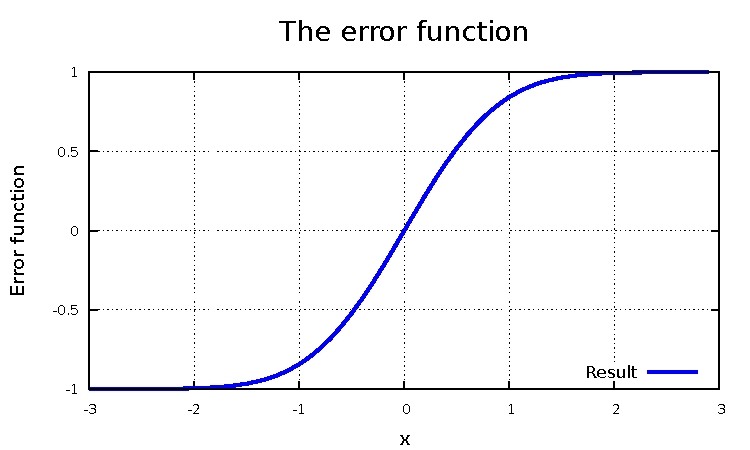
\includegraphics[width = 0.9\columnwidth]{plot_err.pdf}
	\caption{\sl Solution to the error function. For a given random variable following a normal distribution with an expectation value of $0$, and a standard deviation of $0.5$, the error function will show the probability of it being within a range of $[-x;x]$.}
	\label{fig:err_fun}
\end{figure}
The error function has several related functions including the complementary error function defined as 

\begin{equation*}
    erfc(x) = 1  - erf(x),
\end{equation*}

\noindent and the imaginary error function given by the equation

\begin{equation*}
    erfi(x) = - i erf(ix).
\end{equation*}

\noindent As for the mathematical properties, the integrand is an even function - $e^{-t^2}$ - so it is given that the error function is odd. It also has no singularities which means that its Taylor expansion will always converge.
There are also several numerical approximations varying in accuracy given by \textit{Abramowitz} and \textit{Stegun}.
This has been a short introduction of the error function. For a more thorough run-through please see~\cite{mymain}.

\printbibliography

\end{document}
